\subsection{SchedRR vs SchedRR2}

Para comparar el funcionamiento de los dos schedulers simularemos el comportamiento de ambos algoritmos utilizando tres lote de tareas: $lotePc$, $loteCelular$ y $loteCalc$ (explicados anteriormente) con el fin de realizar una experimentación profunda sobre ambos algoritmos.

Para cada uno de los lotes calcularemos el waiting time y turnaround time promedio para cada scheduler tomando distintos valores de quantum y probando con 2, 3 y 4 cores. Los costos de cambio de contexto y migración serán 1 y 2 repectivamente. Teniendo en cuenta los resultados concluiremos cuál de los dos algoritmos se comporta mejor.

\subsubsection{Lote 1: Pc}

\begin{figure}[H]
\hfill
\subfigure[]{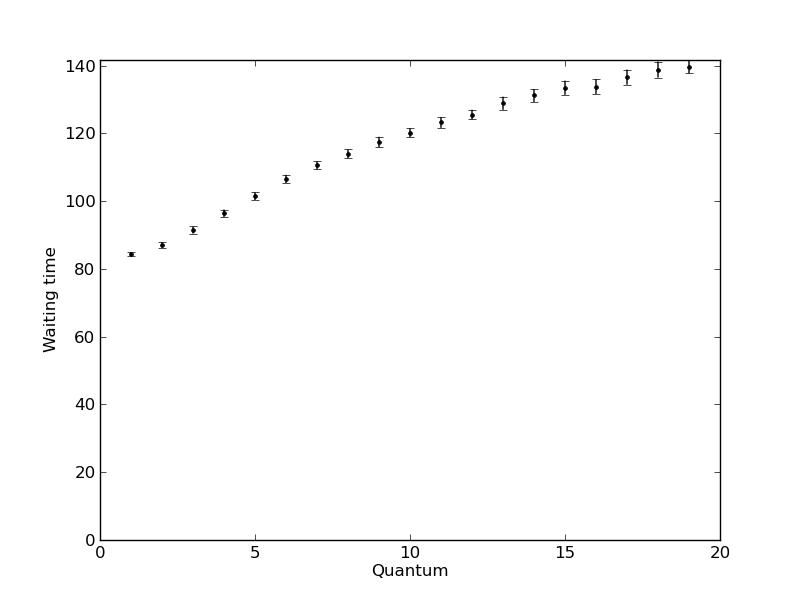
\includegraphics[width=8.75cm]{graficos/schedRR_pc/cores_2_wt.jpg}}
\hfill
\subfigure[]{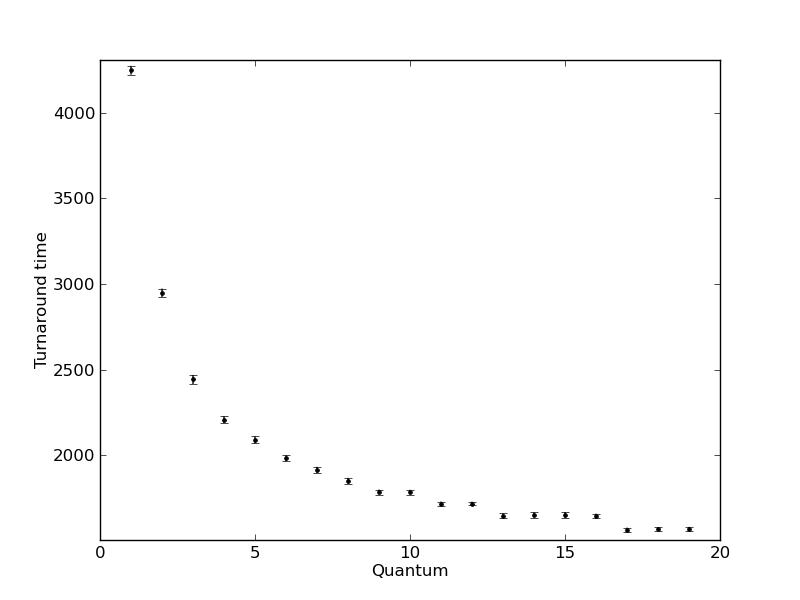
\includegraphics[width=8.75cm]{graficos/schedRR_pc/cores_2_ta.jpg}}
\hfill
\caption{Gráfico de Waiting time y turnaround time en función del quantum con 2 cores para lote de tareas $lotePc$ en SchedRR}
\end{figure}

\begin{figure}[H]
\hfill
\subfigure[]{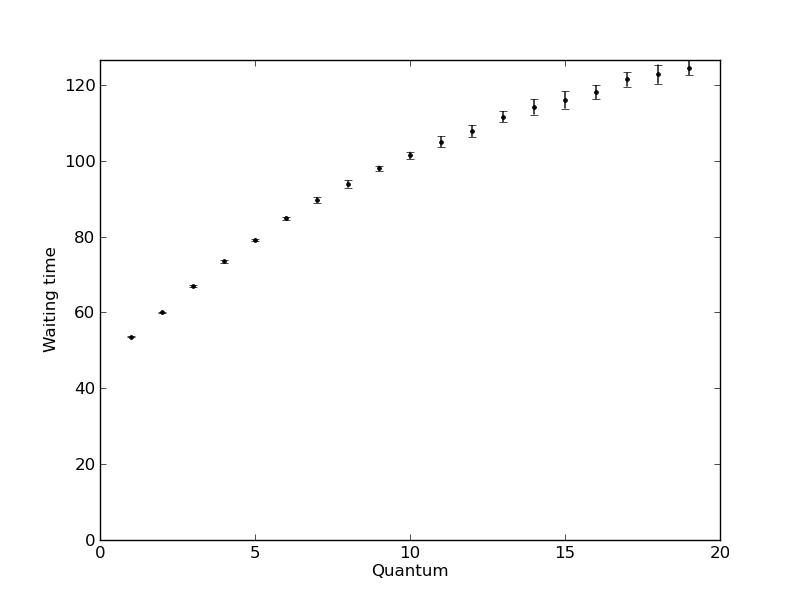
\includegraphics[width=8.75cm]{graficos/schedRR2_pc/cores_2_wt.jpg}}
\hfill
\subfigure[]{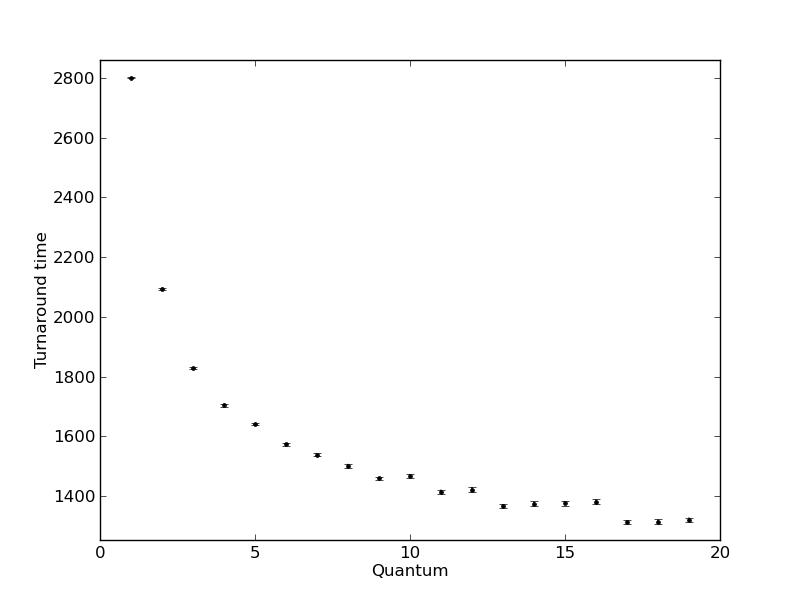
\includegraphics[width=8.75cm]{graficos/schedRR2_pc/cores_2_ta.jpg}}
\hfill
\caption{Gráfico de Waiting time y turnaround time en función del quantum con 2 cores para lote de tareas $lotePc$ en SchedRR2}
\end{figure}

\begin{figure}[H]
\hfill
\subfigure[]{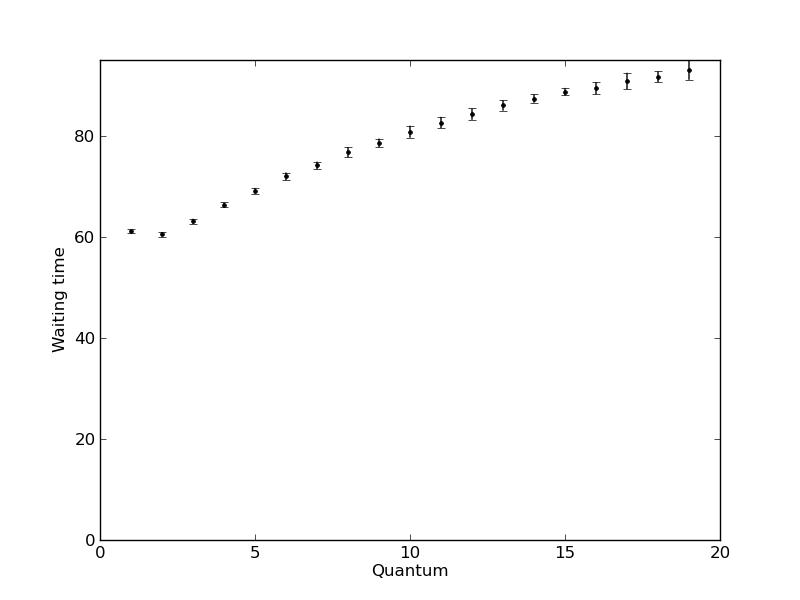
\includegraphics[width=8.75cm]{graficos/schedRR_pc/cores_3_wt.jpg}}
\hfill
\subfigure[]{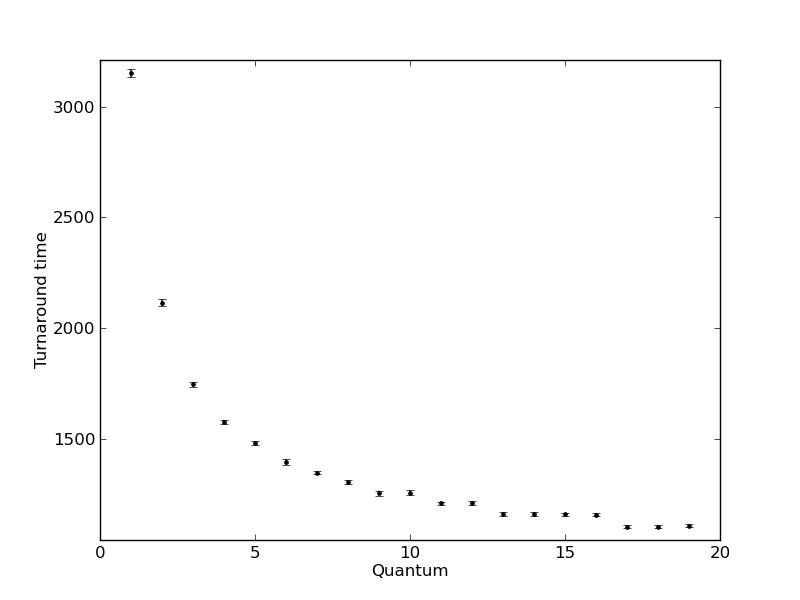
\includegraphics[width=8.75cm]{graficos/schedRR_pc/cores_3_ta.jpg}}
\hfill
\caption{Gráfico de Waiting time y turnaround time en función del quantum con 3 cores para lote de tareas $lotePc$ en SchedRR}
\end{figure}

\begin{figure}[H]
\hfill
\subfigure[]{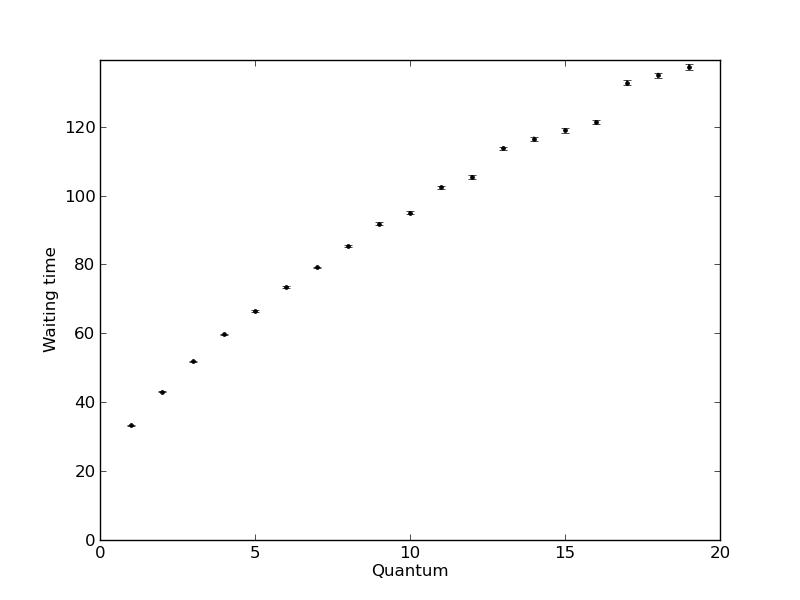
\includegraphics[width=8.75cm]{graficos/schedRR2_pc/cores_3_wt.jpg}}
\hfill
\subfigure[]{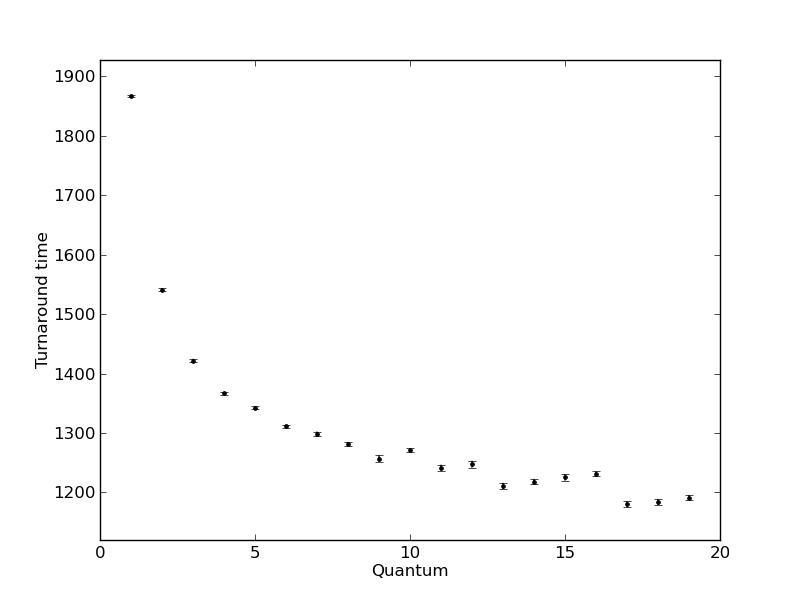
\includegraphics[width=8.75cm]{graficos/schedRR2_pc/cores_3_ta.jpg}}
\hfill
\caption{Gráfico de Waiting time y turnaround time en función del quantum con 3 cores para lote de tareas $lotePc$ en SchedRR2}
\end{figure}

\begin{figure}[H]
\hfill
\subfigure[]{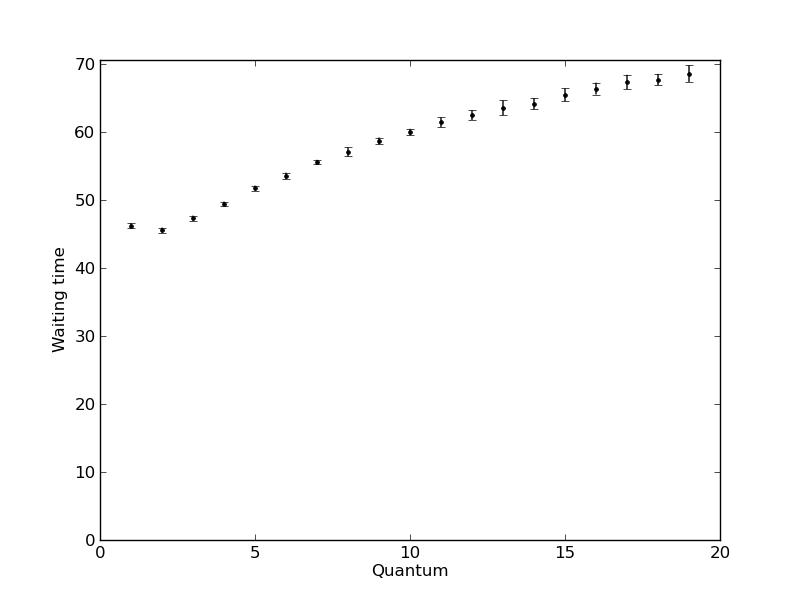
\includegraphics[width=8.75cm]{graficos/schedRR_pc/cores_4_wt.jpg}}
\hfill
\subfigure[]{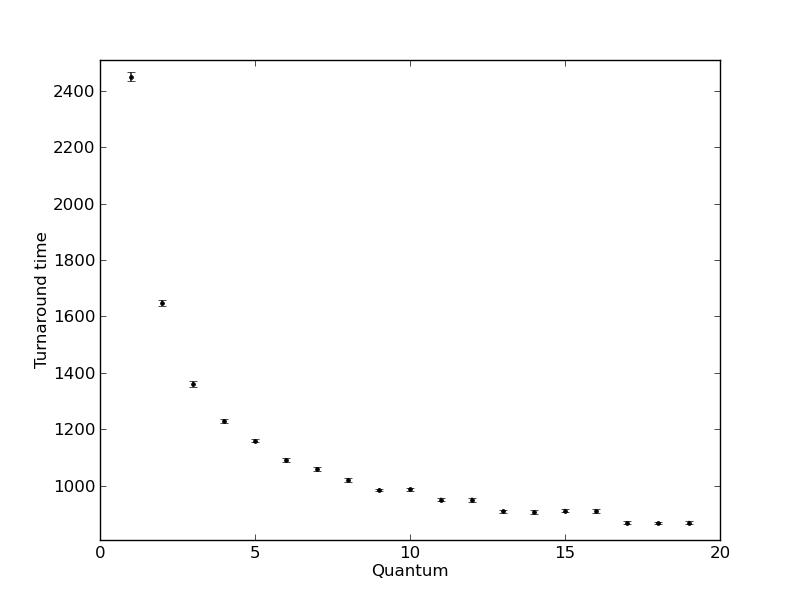
\includegraphics[width=8.75cm]{graficos/schedRR_pc/cores_4_ta.jpg}}
\hfill
\caption{Gráfico de Waiting time y turnaround time en función del quantum con 4 cores para lote de tareas $lotePc$ en SchedRR}
\end{figure}

\begin{figure}[H]
\hfill
\subfigure[]{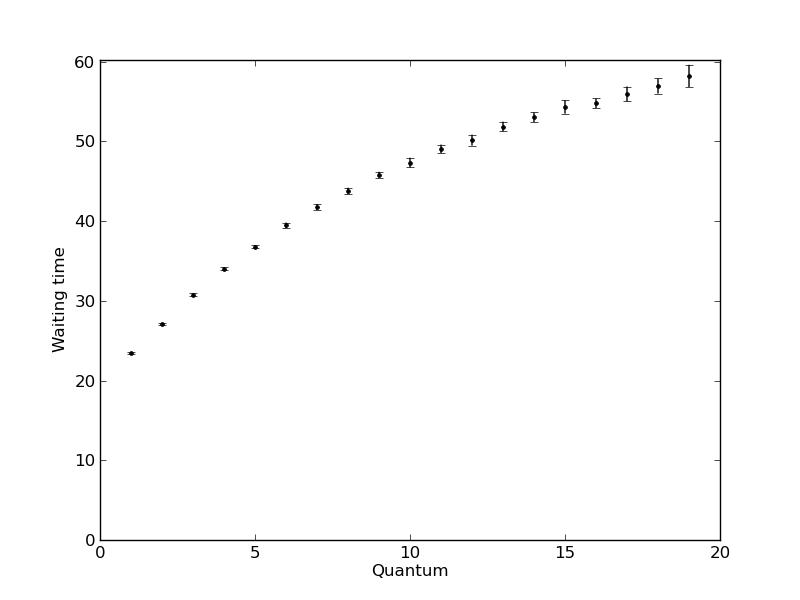
\includegraphics[width=8.75cm]{graficos/schedRR2_pc/cores_4_wt.jpg}}
\hfill
\subfigure[]{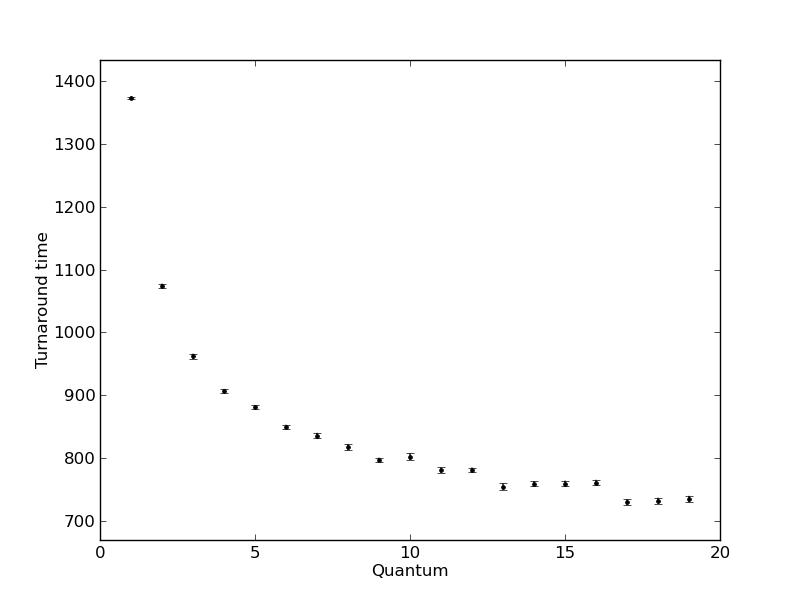
\includegraphics[width=8.75cm]{graficos/schedRR2_pc/cores_4_ta.jpg}}
\hfill
\caption{Gráfico de Waiting time y turnaround time en función del quantum con 4 cores para lote de tareas $lotePc$ en SchedRR2}
\end{figure}

\begin{center}
    \begin{tabular}{ | l | l | l | l | l | p{5cm} |}
    \hline
    Cores & Wt RR & Wt RR2 & Ta RR & Ta RR2 \\ \hline
    2 & 116.89 & 97 & 1998.06 & 1573.38 \\ \hline
    3 & 78.71 & 92.74 & 1420.25 & 1310.04 \\ \hline
    4 & 58.5 & 44.98 & 1112.45 & 847.02 \\
	\hline
    \end{tabular}
\captionof{table}{Waiting time y Turnaround time promedio para cada scheduler}
\end{center}

Observando la tabla podemos concluir que el schedRR2 tiene un mejor wt y ta en promedio para un lote de tareas pc.

\subsubsection{Lote 2: celular}

\begin{figure}[H]
\hfill
\subfigure[]{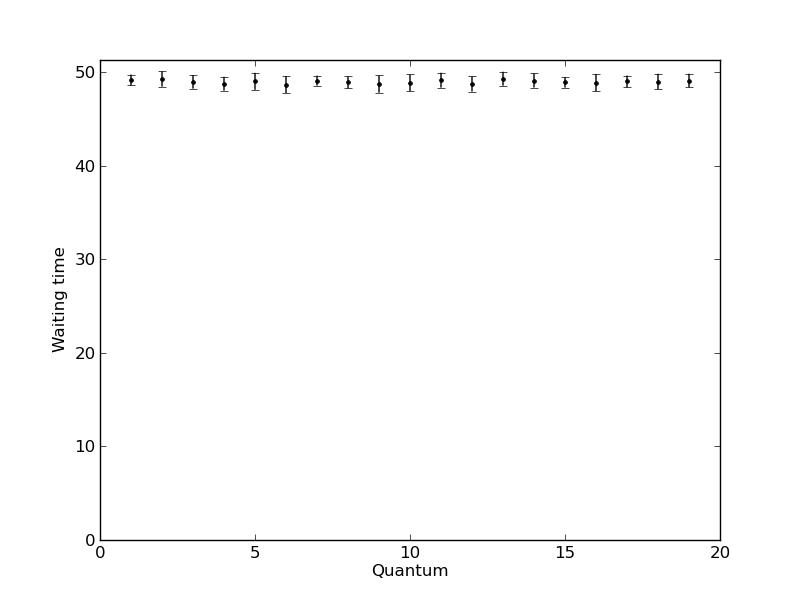
\includegraphics[width=8.75cm]{graficos/schedRR_celular/cores_2_wt.jpg}}
\hfill
\subfigure[]{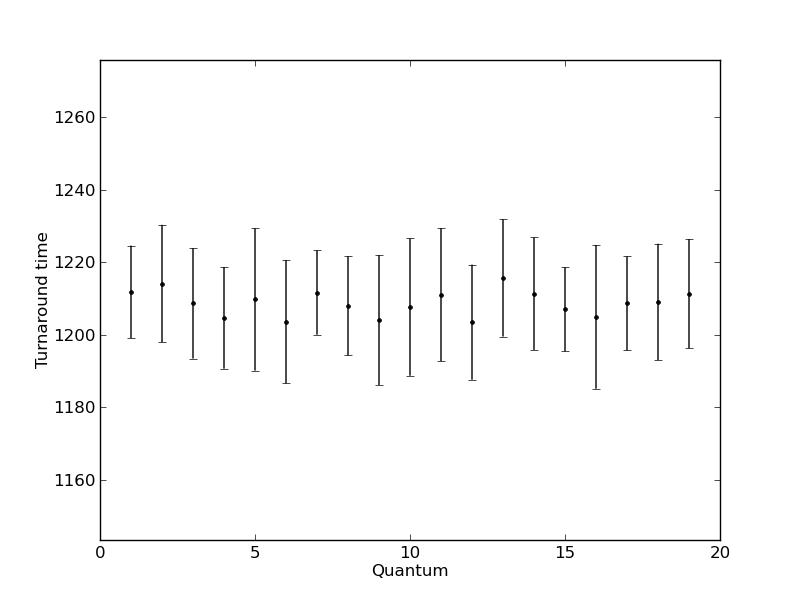
\includegraphics[width=8.75cm]{graficos/schedRR_celular/cores_2_ta.jpg}}
\hfill
\caption{Gráfico de Waiting time y turnaround time en función del quantum con 2 cores para lote de tareas $loteCelular$ en SchedRR}
\end{figure}

\begin{figure}[H]
\hfill
\subfigure[]{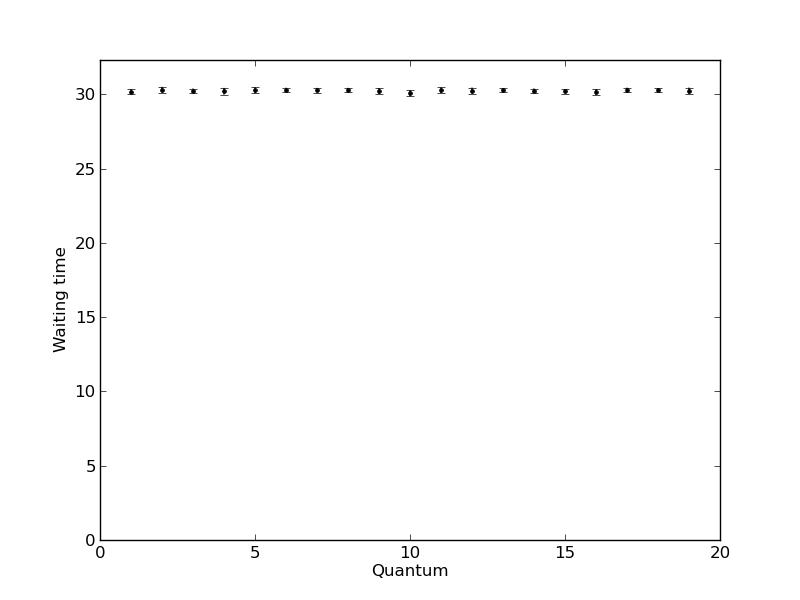
\includegraphics[width=8.75cm]{graficos/schedRR2_celular/cores_2_wt.jpg}}
\hfill
\subfigure[]{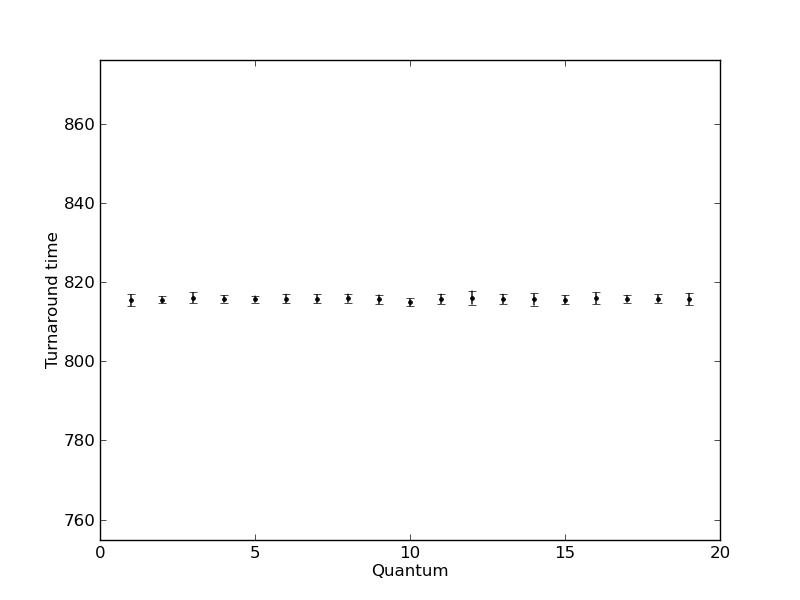
\includegraphics[width=8.75cm]{graficos/schedRR2_celular/cores_2_ta.jpg}}
\hfill
\caption{Gráfico de Waiting time y turnaround time en función del quantum con 2 cores para lote de tareas $loteCelular$ en SchedRR2}
\end{figure}

\begin{figure}[H]
\hfill
\subfigure[]{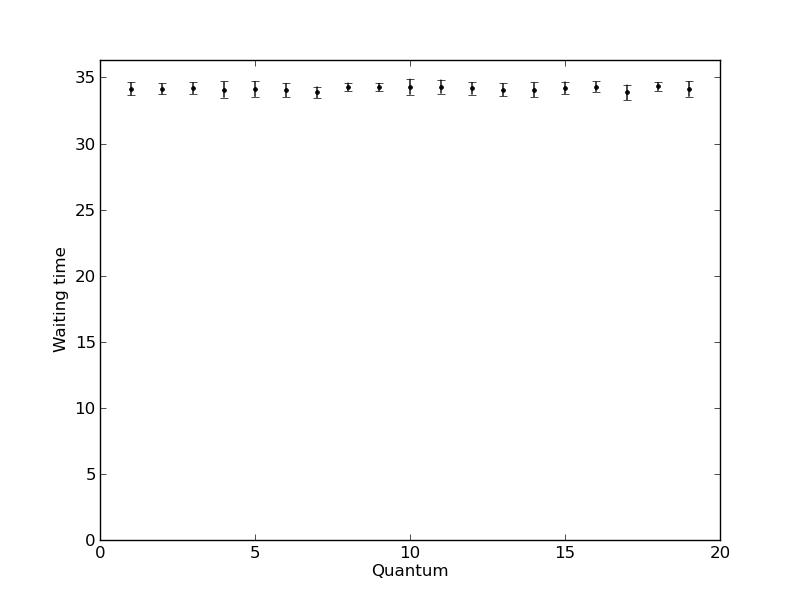
\includegraphics[width=8.75cm]{graficos/schedRR_celular/cores_3_wt.jpg}}
\hfill
\subfigure[]{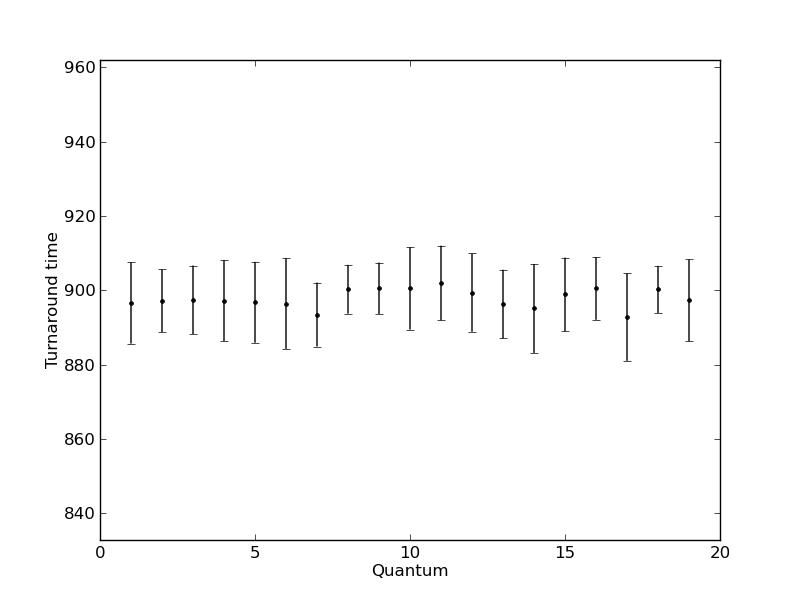
\includegraphics[width=8.75cm]{graficos/schedRR_celular/cores_3_ta.jpg}}
\hfill
\caption{Gráfico de Waiting time y turnaround time en función del quantum con 3 cores para lote de tareas $loteCelular$ en SchedRR}
\end{figure}

\begin{figure}[H]
\hfill
\subfigure[]{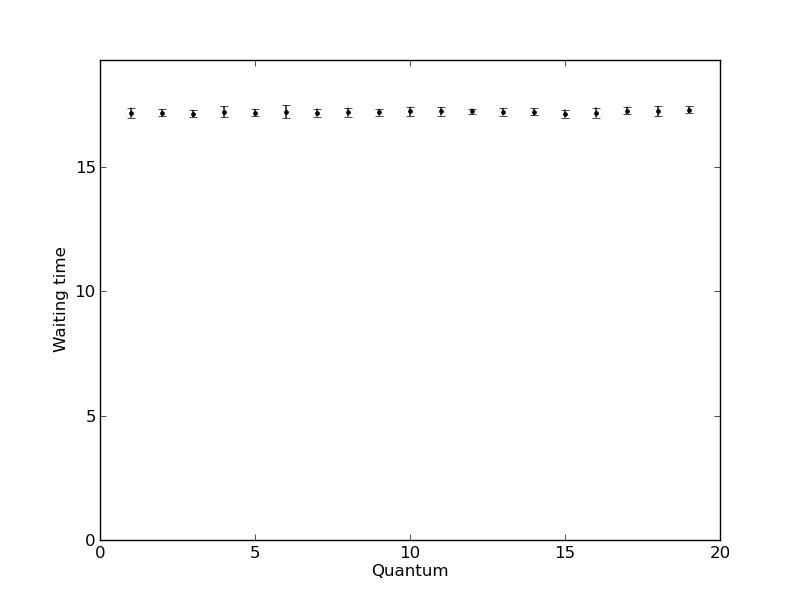
\includegraphics[width=8.75cm]{graficos/schedRR2_celular/cores_3_wt.jpg}}
\hfill
\subfigure[]{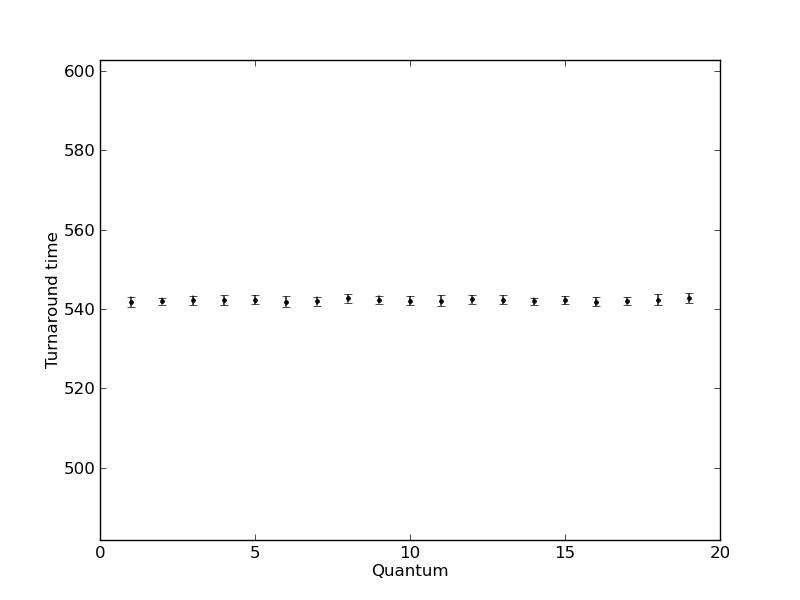
\includegraphics[width=8.75cm]{graficos/schedRR2_celular/cores_3_ta.jpg}}
\hfill
\caption{Gráfico de Waiting time y turnaround time en función del quantum con 3 cores para lote de tareas $loteCelular$ en SchedRR2}
\end{figure}

\begin{figure}[H]
\hfill
\subfigure[]{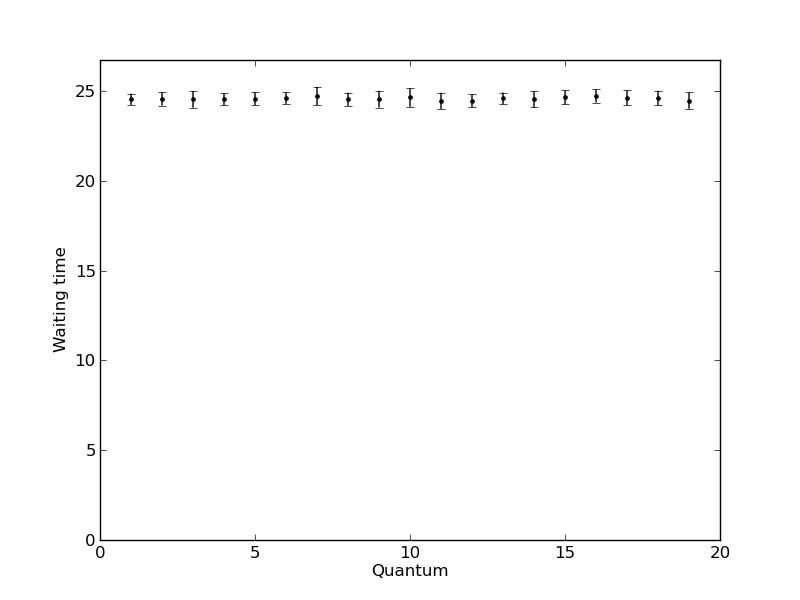
\includegraphics[width=8.75cm]{graficos/schedRR_celular/cores_4_wt.jpg}}
\hfill
\subfigure[]{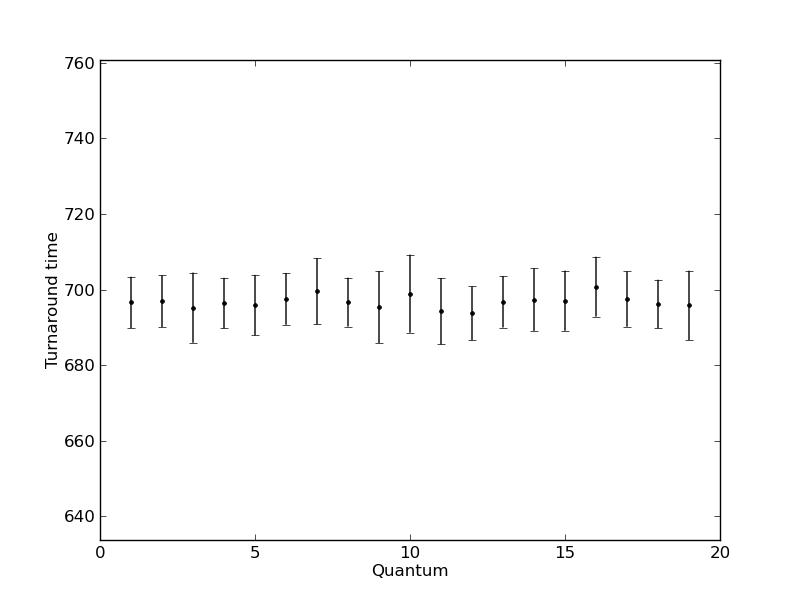
\includegraphics[width=8.75cm]{graficos/schedRR_celular/cores_4_ta.jpg}}
\hfill
\caption{Gráfico de Waiting time y turnaround time en función del quantum con 4 cores para lote de tareas $loteCelular$ en SchedRR}
\end{figure}

\begin{figure}[H]
\hfill
\subfigure[]{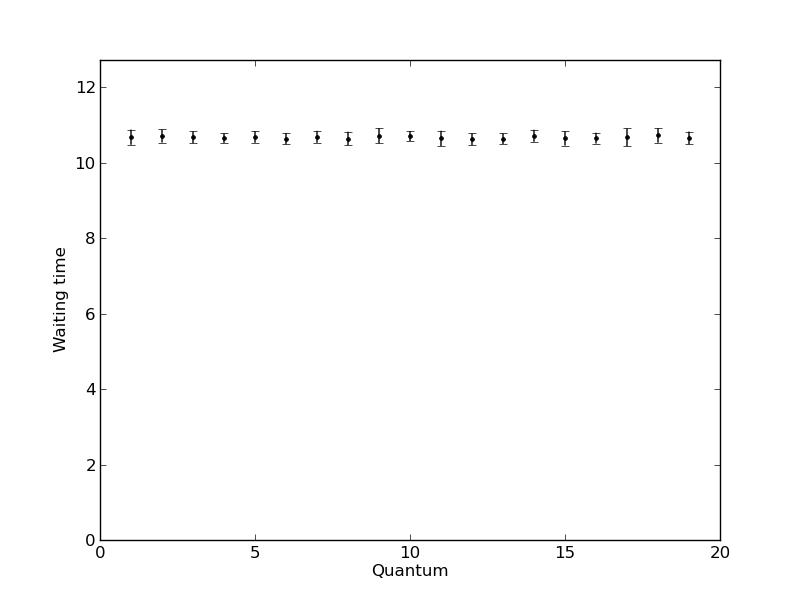
\includegraphics[width=8.75cm]{graficos/schedRR2_celular/cores_4_wt.jpg}}
\hfill
\subfigure[]{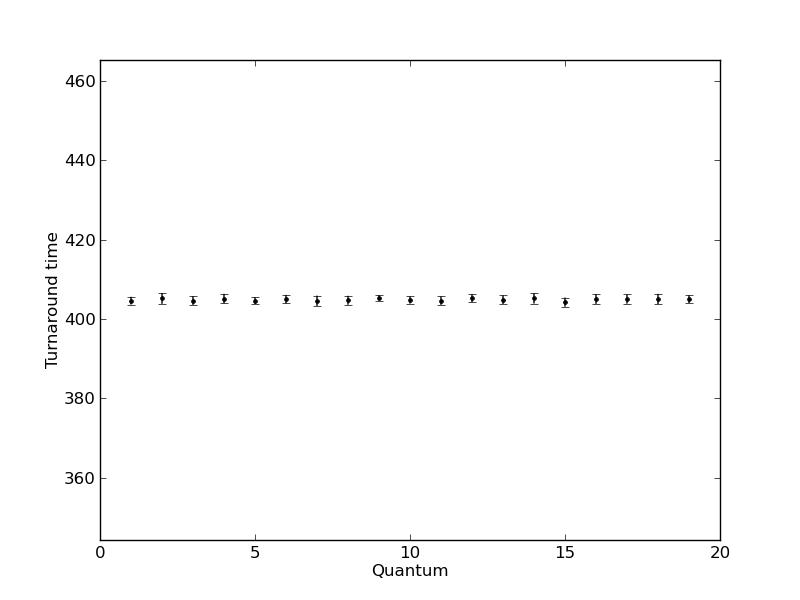
\includegraphics[width=8.75cm]{graficos/schedRR2_celular/cores_4_ta.jpg}}
\hfill
\caption{Gráfico de Waiting time y turnaround time en función del quantum con 4 cores para lote de tareas $loteCelular$ en SchedRR2}
\end{figure}

\begin{center}
    \begin{tabular}{ | l | l | l | l | l | p{5cm} |}
    \hline
    Cores & Wt RR & Wt RR2 & Ta RR & Ta RR2 \\ \hline
    2 & 48.96 & 30.25 & 1208.74 & 815.69 \\ \hline
    3 & 34.15 & 17.20 & 897.83 & 542.165 \\ \hline
    4 & 24.58 & 10.67 & 696.76 & 404.9 \\
	\hline
    \end{tabular}
\captionof{table}{Waiting time y Turnaround time promedio para cada scheduler}
\end{center}

Observando la tabla podemos concluir que el schedRR2 tiene un mejor wt y ta en promedio para un lote de tareas celular.

\subsubsection{Lote 3: uso intensivo de CPU}

\begin{figure}[H]
\hfill
\subfigure[]{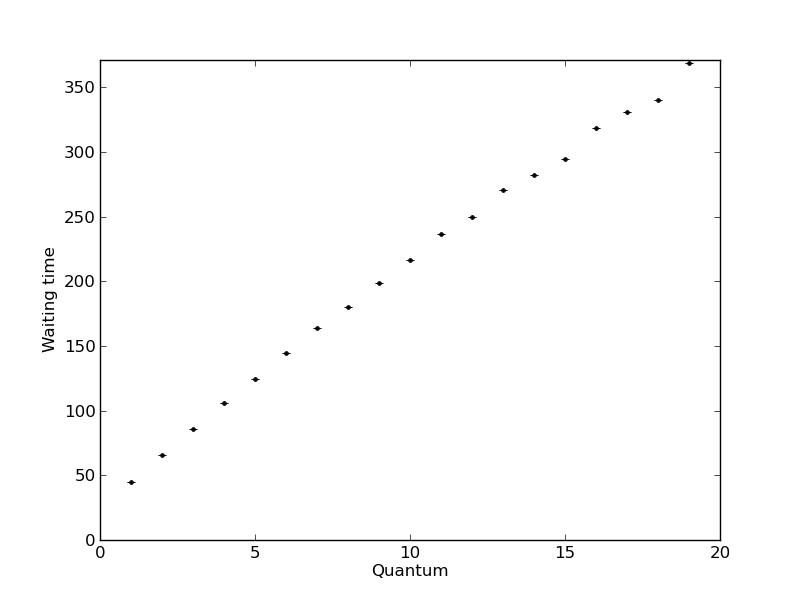
\includegraphics[width=8.75cm]{graficos/schedRR_cpu/cores_2_wt.jpg}}
\hfill
\subfigure[]{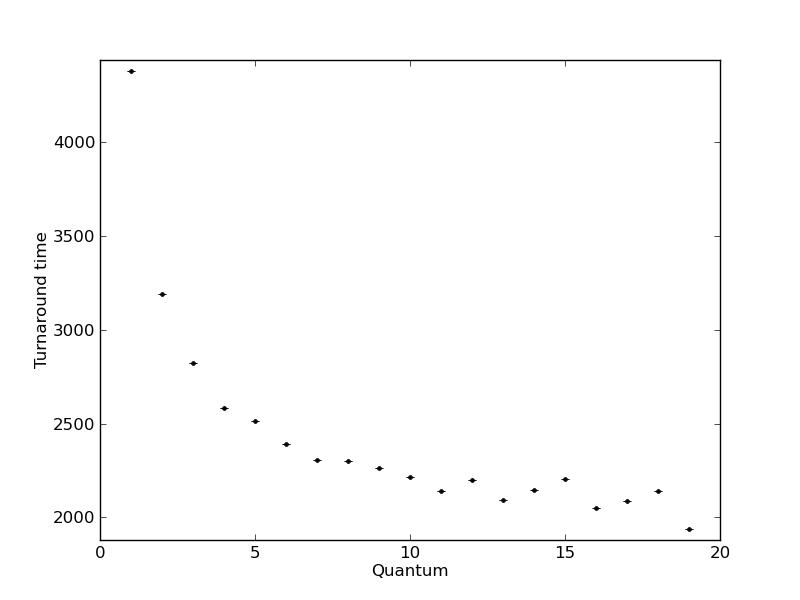
\includegraphics[width=8.75cm]{graficos/schedRR_cpu/cores_2_ta.jpg}}
\hfill
\caption{Gráfico de Waiting time y turnaround time en función del quantum con 2 cores para lote de tareas $loteCpu$ en SchedRR}
\end{figure}

\begin{figure}[H]
\hfill
\subfigure[]{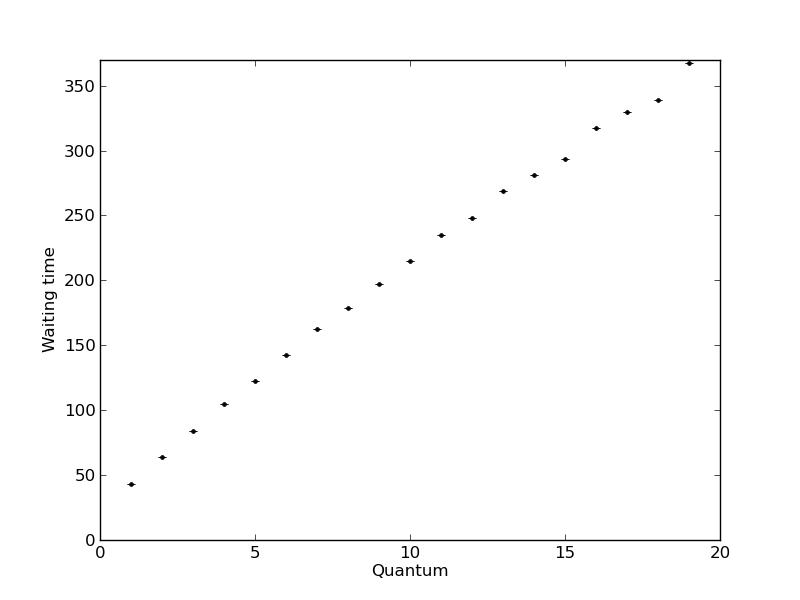
\includegraphics[width=8.75cm]{graficos/schedRR2_cpu/cores_2_wt.jpg}}
\hfill
\subfigure[]{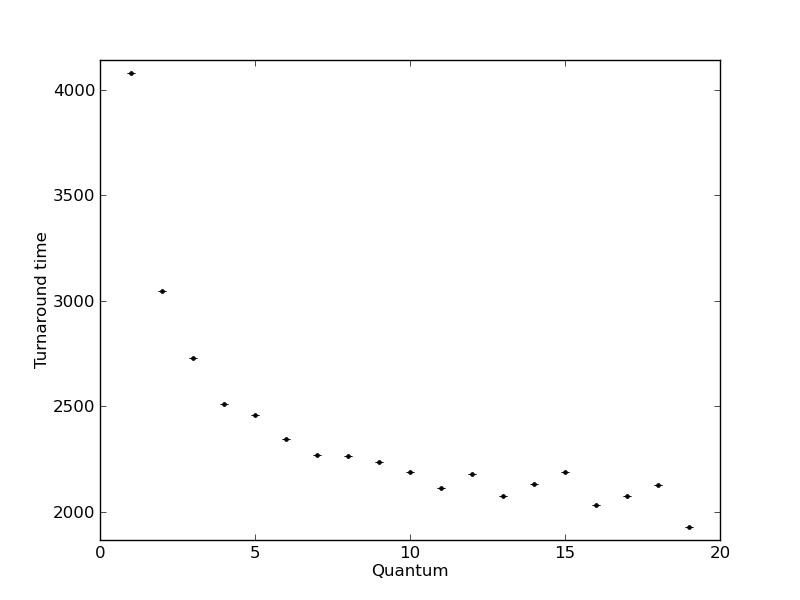
\includegraphics[width=8.75cm]{graficos/schedRR2_cpu/cores_2_ta.jpg}}
\hfill
\caption{Gráfico de Waiting time y turnaround time en función del quantum con 2 cores para lote de tareas $loteCpu$ en SchedRR2}
\end{figure}

\begin{figure}[H]
\hfill
\subfigure[]{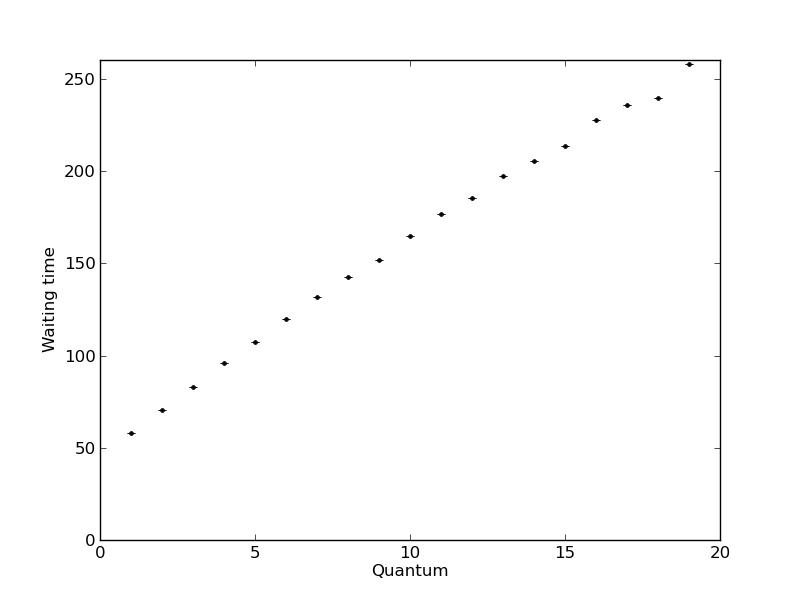
\includegraphics[width=8.75cm]{graficos/schedRR_cpu/cores_3_wt.jpg}}
\hfill
\subfigure[]{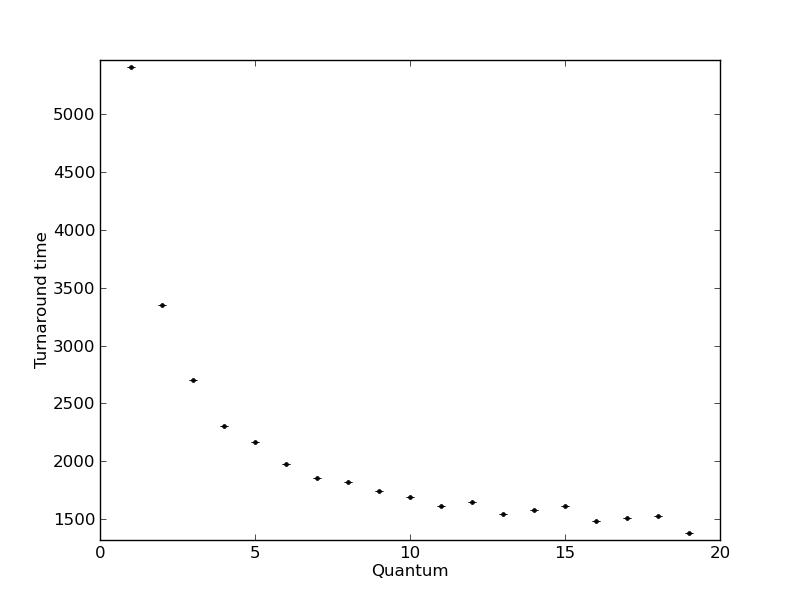
\includegraphics[width=8.75cm]{graficos/schedRR_cpu/cores_3_ta.jpg}}
\hfill
\caption{Gráfico de Waiting time y turnaround time en función del quantum con 3 cores para lote de tareas $loteCpu$ en SchedRR}
\end{figure}

\begin{figure}[H]
\hfill
\subfigure[]{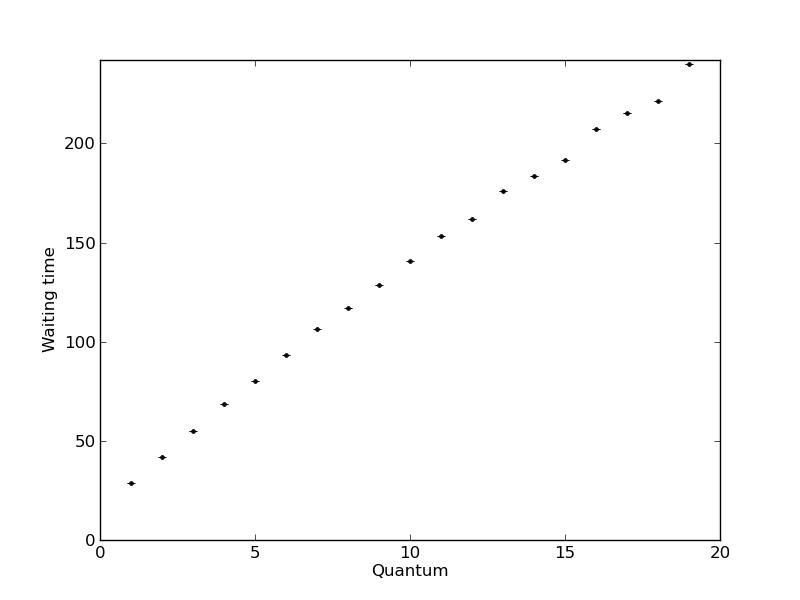
\includegraphics[width=8.75cm]{graficos/schedRR2_cpu/cores_3_wt.jpg}}
\hfill
\subfigure[]{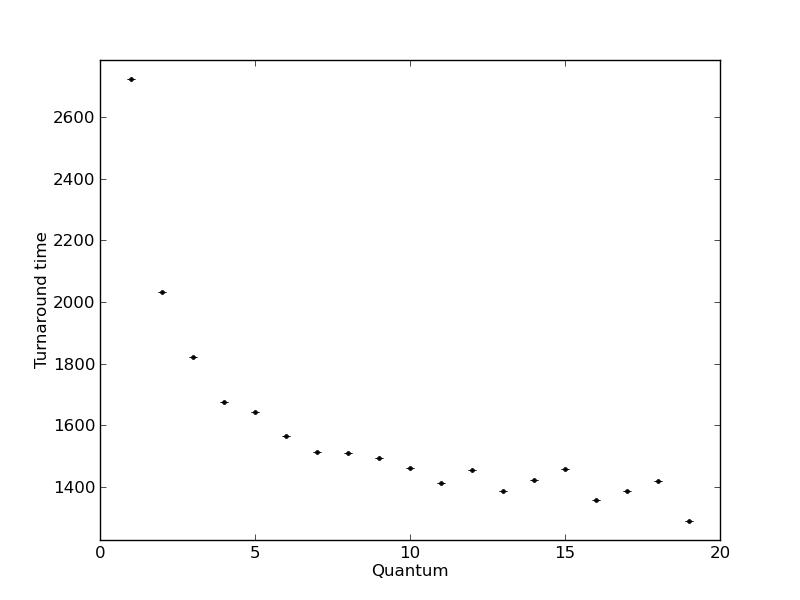
\includegraphics[width=8.75cm]{graficos/schedRR2_cpu/cores_3_ta.jpg}}
\hfill
\caption{Gráfico de Waiting time y turnaround time en función del quantum con 3 cores para lote de tareas $loteCpu$ en SchedRR2}
\end{figure}

\begin{figure}[H]
\hfill
\subfigure[]{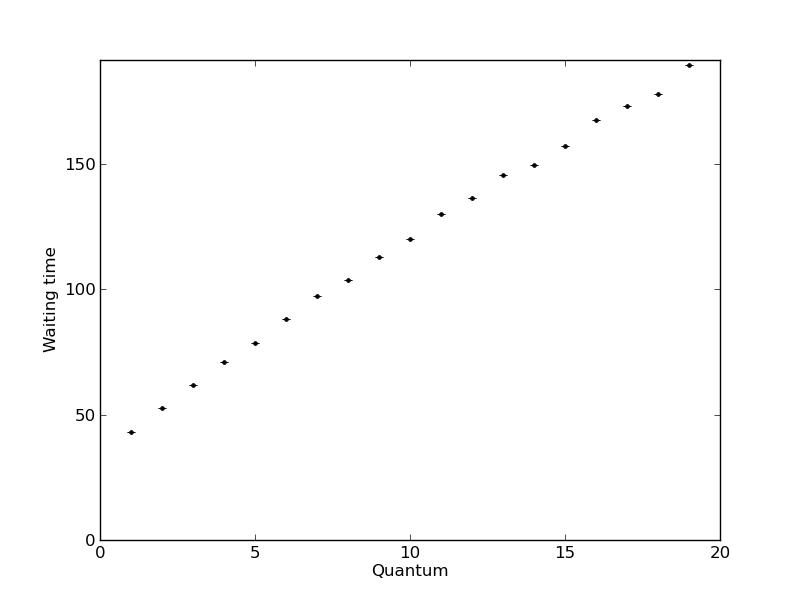
\includegraphics[width=8.75cm]{graficos/schedRR_cpu/cores_4_wt.jpg}}
\hfill
\subfigure[]{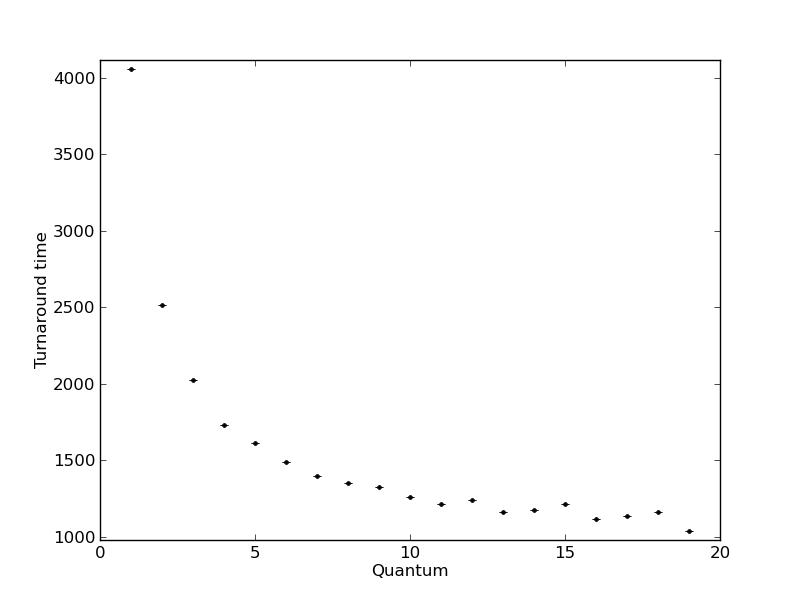
\includegraphics[width=8.75cm]{graficos/schedRR_cpu/cores_4_ta.jpg}}
\hfill
\caption{Gráfico de Waiting time y turnaround time en función del quantum con 4 cores para lote de tareas $loteCpu$ en SchedRR}
\end{figure}

\begin{figure}[H]
\hfill
\subfigure[]{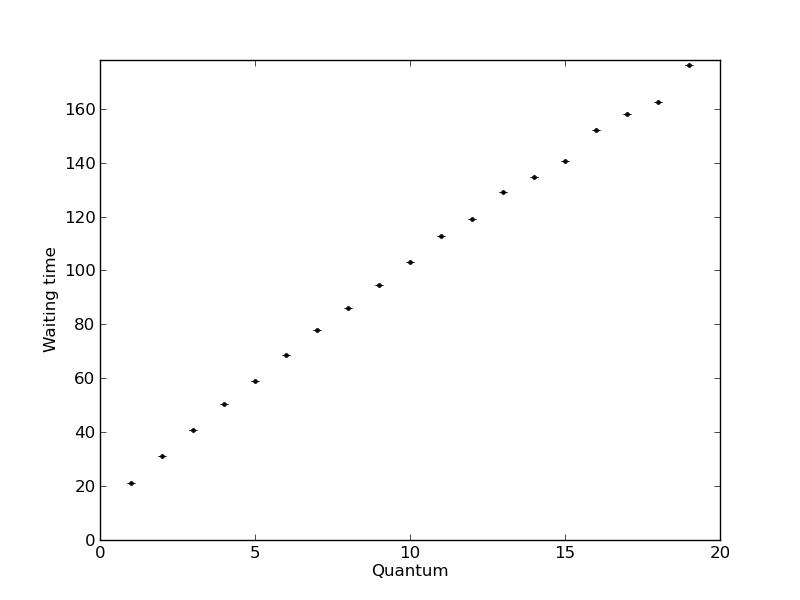
\includegraphics[width=8.75cm]{graficos/schedRR2_cpu/cores_4_wt.jpg}}
\hfill
\subfigure[]{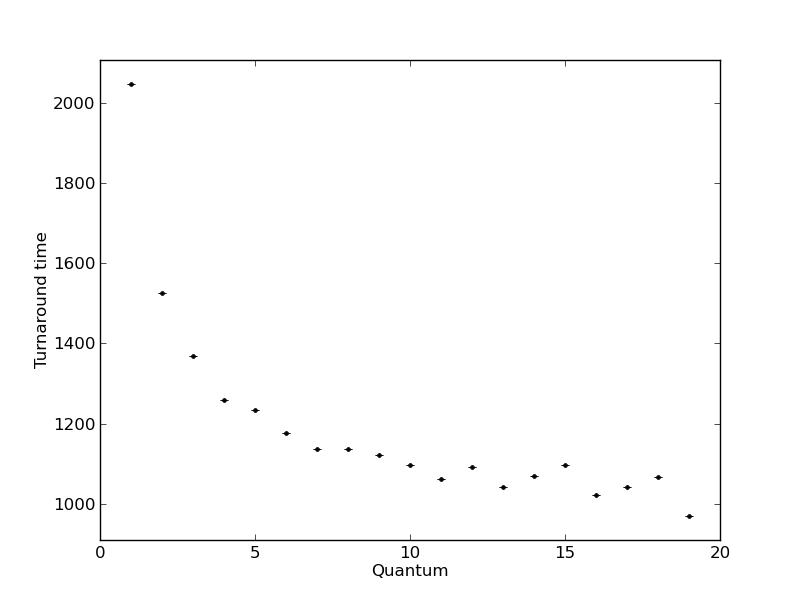
\includegraphics[width=8.75cm]{graficos/schedRR2_cpu/cores_4_ta.jpg}}
\hfill
\caption{Gráfico de Waiting time y turnaround time en función del quantum con 4 cores para lote de tareas $loteCpu$ en SchedRR2}
\end{figure}

\begin{center}
    \begin{tabular}{ | l | l | l | l | l | p{5cm} |}
    \hline
    Cores & Wt RR & Wt RR2 & Ta RR & Ta RR2 \\ \hline
    2 & 211.64 & 210.27 & 2419.82 & 2365.98 \\ \hline
    3 & 161.31 & 137.4 & 2049.82 & 1580.55 \\ \hline
    4 & 118.75 & 100.94 & 1537.24 & 1187.93 \\
	\hline
    \end{tabular}
\captionof{table}{Waiting time y Turnaround time promedio para cada scheduler}
\end{center}

Observando la tabla podemos concluir que el schedRR2 tiene un mejor wt y ta en promedio para un lote de tareas de uso intensivo de CPU.

En conclusión, podemos afirmar que el scheduler Round Robin que no permite migración de procesos entre núcleos (SchedRR2) funciona mejor que el SchedRR teniendo en cuenta las métricas de Turnaround time y Waiting time. Creemos que la diferencia de performance entre ambos schedulers radica en el hecho de que el SchedRR2 se ahorra los costos de migración cada vez que cambia de tarea.

